\documentclass[a4paper,11pt,dvipdfmx]{jsarticle}


% 数式
\usepackage{amsmath,amsfonts}
\usepackage{bm}

% 画像
\usepackage[dvipdfmx]{graphicx}
\usepackage{framed}

% 図形
\usepackage{tikz}
\usetikzlibrary{shapes.geometric}
\usetikzlibrary {shapes.misc}

% ソースコード
\usepackage{listings,jlisting,color}
\lstset{
language={C},
backgroundcolor={\color[gray]{.85}},
basicstyle={\ttfamily},
identifierstyle={\small},
commentstyle={\smallitshape \color[rgb]{0,0.5,0}},
keywordstyle={\small\bfseries \color[rgb]{1,0,0}},
ndkeywordstyle={\small},
stringstyle={\small\ttfamily \color[rgb]{0,0,1}},
frame={tb},
breaklines=true,
columns=[l]{fullflexible},
numbers=left,
xrightmargin=0zw,
xleftmargin=3zw,
numberstyle={\scriptsize},
stepnumber=1,
numbersep=1zw,
lineskip=-0.5ex,
morecomment=[l]{//}
}
\renewcommand{\lstlistingname}{ソースコード}


\begin{document}
\definecolor{shadecolor}{gray}{0.70}

\title{最適化 Class-2 演習}
\author{21T2166D 渡辺大樹}
\date{\today}
\maketitle

\section{演習内容}
Class-2では探索における最適化を、関数の最大値を求めるアルゴリズムの設計を用いて理解していく。

今回用いるアルゴリズムは全探索と山登り探索になる。
全探索は決められた定義域における関数の値をすべて求め、そこから最大の値となる関数の値と引数を特定する方法になる。

山登り探索はある初期値から関数の値が大きくなる方へ山に登るように移動し、最大となった点の関数の値と引数を返す方法になる。

この二つの探索を1変数関数と2変数関数で行っていく。
実装したコードはソースコード\ref{ex},\ref{hill},\ref{ex3d},\ref{hill3d}に示す。コードがかなり長いためレポート末に示す。

\subsection{1変数関数での探索}
最大値を求める関数は(1)(2)の2種類を用いる。
\begin{align}
    f(x) &= \sin(x)\\
    g(x) &= \frac{\sin(x^3-5(x+0.1)^2)}{x^3+(x+0.1)^{-2}}
\end{align}

この二つの関数について、ある区間$[x_{min},x_{max}]$においての最大値を求めるアルゴリズムを示していく。

全探索では探索する間隔となる$delta$を用いて$[x_{min},x_{max}]$を
この$delta$で分割したすべての$x$の値において$f(x)$を計算する。
この$x$での関数の出力値が$x-delta$の出力値よりも大きい場合にのみ、
その関数値と$x$の値をそれぞれ$fbest,xbest$で保存する。

これにより区間すべての探索が終わった際、保存されていた$fbest,xbest$がこの区間での関数の最大値となる。

山登り探索では探索する間隔$delta$と探索の初期値$x_0$を設定する。
まずその探索にあたって探索の初期値から$\pm delta$分離れた関数の値と初期値での関数の値
$f(x_0-delta),f(x_0),f(x_0+delta)$を用意する。
この3つの関数の値を比較することで、グラフのいわば登るべき方向を決めることができる。
$f(x_0-delta)$が大きければ$x$の負の方向に探索を進め、$f(x_0+delta)$が大きければ$x$の正の方向に探索を進める。
$f(x_0)$が大きいとその点が極大値となり、探索は終了する。
ここで決めた方向は$sign$に$\pm1$の値で保存され、$delta$に掛けてから$x$の値に足し算することで探索が進行する。

以降は$f(x)$と$f(x+delta)$の値を比較していき、$f(x+delta)$が大きい場合は探索を続行し、
$f(x)$の値が大きくなる場合はその点が極大値となるため、探索はそこで終了する。

これにより探索終了時の$x$と$f(x)$が出力される。

\subsection{2変数関数での探索}
最大値を求める関数は(3)(4)の2種類を用いる。
\begin{align}
    f(x_1,x_2) &= \frac{1}{2} (\sin(x_1) + \sin(x_2))\\
    g(x_1,x_2) &= \frac{1}{2} \left( \frac{\sin({x_1}^3-5(x_1+0.1)^2)}{{x_1}^3+(x_1+0.1)^{-2}} + \frac{\sin({x_2}^3-5(x_2+0.1)^2)}{{x_2}^3+(x_2+0.1)^{-2}} \right)
\end{align}

2変数関数であっても基本行うことは変わらない。そのためここでは相違点を示していく。
最大値を求める区間は$[[x_{(1)min},x_{(2)min}],[x_{(1)max},x_{(2)max}]]$となる。
全探索ではこの区間すべてにおいて探索間隔$delta$を用いて関数値$f(x_1,x_2)$を計算し、最大値を探す。

山登り探索では探索の初期値$(x_{(1)0},x_{(2)0})$と探索する間隔$delta$を同様に用意する。
変更点は探索を始める際に決める探索の向きで、1変数の際は$x$に対して正負どちらかの方向、
もしくはその場が最大値となっていたが、2変数となるので$x_1,x_2$どちらに対しても$\pm delta$したときの
関数値がどうなるかを考えなければならないため、9通りの進行方向が生まれる。

これを変更点としてソースコード\ref{hill}を\ref{hill3d}に変更している。

\section{演習結果}
以下に演習を行った結果を示す。
\subsection{1変数関数での探索}
\subsubsection{全探索}
以下ではソースコード\ref{ex}を実行したときの結果を示す。

始めに関数として(1)式を用い、探索の間隔を$0.01$、探索範囲を$[0,\pi]$としたときの結果が図\ref{es0p0.01}となる。
\begin{figure}[h]
    \centering
    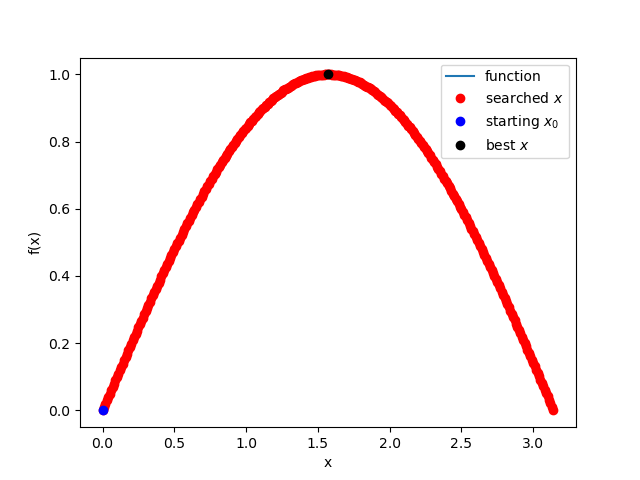
\includegraphics[width=80mm]{c:/program_code/LaTeX/OPT/class2/exsearch_sin_0_3.141592653589793_0.01.png}
    \caption{(1)式を探索間隔$0.01$,探索範囲$[0,\pi]$で全探索を行った結果}
    \label{es0p0.01}
\end{figure}

計算回数は315回で得られた最大値は$f(1.5700000000000012)=0.9999996829318346$となった。
$\sin(x)$は$\frac{\pi}{2}$で最大値1を取るためおおよそ正確な値を得られている。

また探索範囲はそのままで探索の間隔を$0.001$と小さくすると計算回数3142回で得られた最大値は
$f(1.5709999999999378)=0.9999999792586128$となった。理論値との誤差を比較するとおおよそ$\frac{1}{10}$
ほど小さくなっているが計算回数が10倍と多くなってしまっている。

続いて探索する関数として(2)式を用いる。先ほどと同様探索の間隔を$0.01$、探索範囲を$[0,\pi]$としたときの結果が図\ref{ep0p0.01}となる。
\begin{figure}[h]
    \centering
    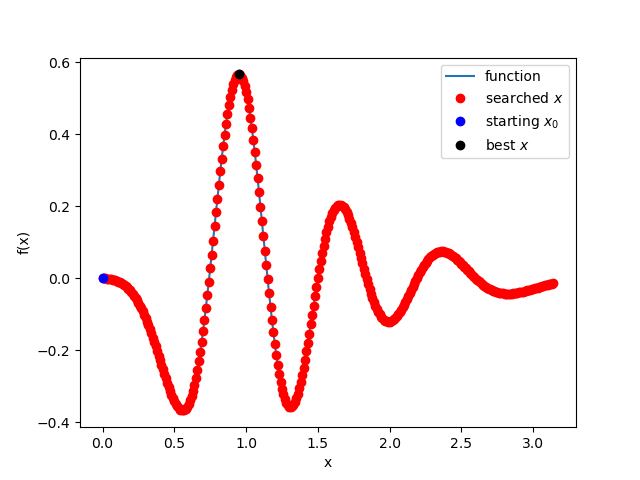
\includegraphics[width=80mm]{c:/program_code/LaTeX/OPT/class2/exsearch_p3d_0_3.141592653589793_0.01.png}
    \caption{(2)式を探索間隔$0.01$,探索範囲$[0,\pi]$で全探索を行った結果}
    \label{ep0p0.01}
\end{figure}

計算回数は315回で得られた最大値は$f(0.9500000000000006)=0.5658344662199044$となった。
すなわちおおよそ$x=0.95$で最大値となる。

このまま探索間隔を$0.001$にすることで得られた最大値は$f(0.9480000000000007)=0.5658822614470929$となった。
計算回数は例によって10倍の3142回であった。

\subsubsection{山登り探索}
以下ではソースコード\ref{hill}を実行したときの結果を示す。

2.1.1と同様、初めに関数として(1)式を用いて、探索間隔を$0.01$、探索範囲を$[0,\pi]$、探索の初期値を$0.6$としたときの結果が図\ref{hs0p0.010.6}となる。
\begin{figure}[h]
    \centering
    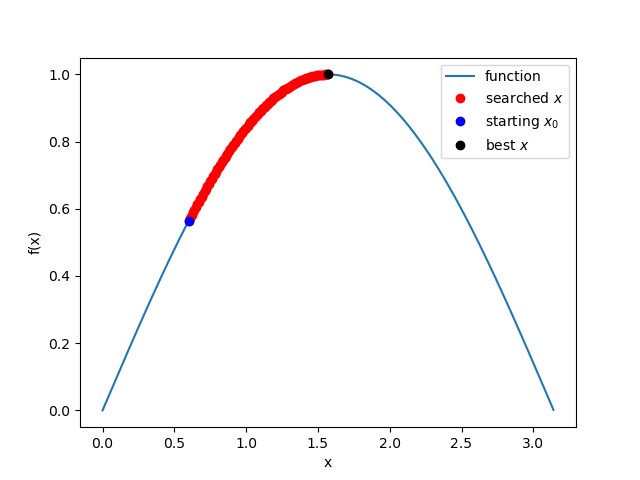
\includegraphics[width=80mm]{c:/program_code/LaTeX/OPT/class2/hillclimib_sin_0_3.141592653589793_0.01_0.6.png}
    \caption{(1)式を探索間隔$0.01$,探索範囲$[0,\pi]$,初期値$0.6$で山登り探索を行った結果}
    \label{hs0p0.010.6}
\end{figure}

図\ref{hs0p0.010.6}では2.1.1での結果と異なり、設定した初期値からの関数の値が大きいほうへの探索となっていることが分かる。
計算回数も出力されたCSVファイルから95回と分かり、格段に計算回数が抑えられていることが分かる。

続いて同様に探索する関数として(2)式を用いる。先ほどと同様探索の間隔を$0.01$、探索範囲を$[0,\pi]$、探索の初期値を$0.6$としたときの結果が図\ref{hp0p0.010.6}となる。
\begin{figure}[h]
    \centering
    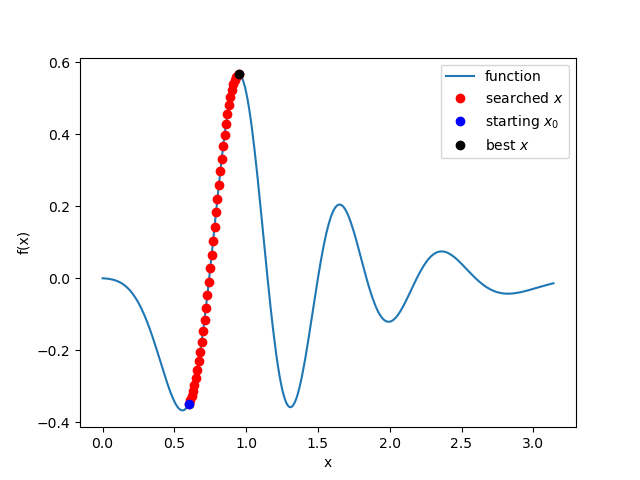
\includegraphics[width=80mm]{c:/program_code/LaTeX/OPT/class2/hillclimib_p3d_0_3.141592653589793_0.01_0.6.png}
    \caption{(2)式を探索間隔$0.01$,探索範囲$[0,\pi]$,初期値$0.6$で山登り探索を行った結果}
    \label{hp0p0.010.6}
\end{figure}

こちらも2.1.1の結果と異なり、初期値から関数の値が大きくなるほうへの探索がされている。
計算回数は34回で、この範囲の最大値となる$x$が0.95と近くなっていることからも計算回数が抑えられている。

初期値を$1.2$に変更すると図\ref{hp0p0.011.2}となる。
\begin{figure}[h]
    \centering
    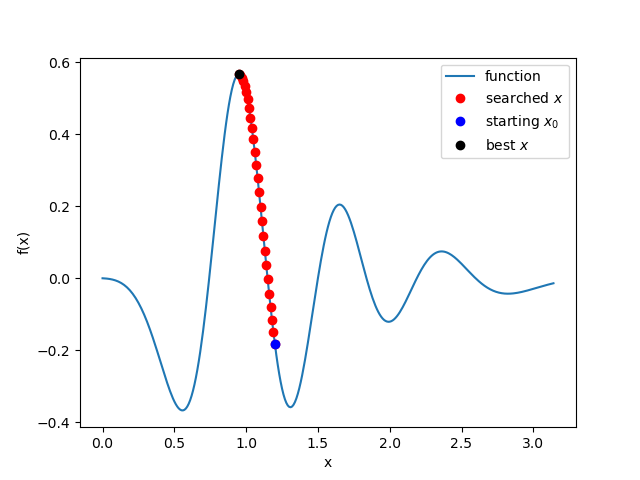
\includegraphics[width=80mm]{c:/program_code/LaTeX/OPT/class2/hillclimib_p3d_0_3.141592653589793_0.01_1.2.png}
    \caption{(2)式を探索間隔$0.01$,探索範囲$[0,\pi]$,初期値$1.2$で山登り探索を行った結果}
    \label{hp0p0.011.2}
\end{figure}

この図を見るとよくわかるが山登りでの探索のため初期値を変化させても関数の値が大きくなるほうへ$x$の値が変わっていることが分かる。

また初期値を$1.5$に変更すると図\ref{hs0p0.011.5}となる。
\begin{figure}[h]
    \centering
    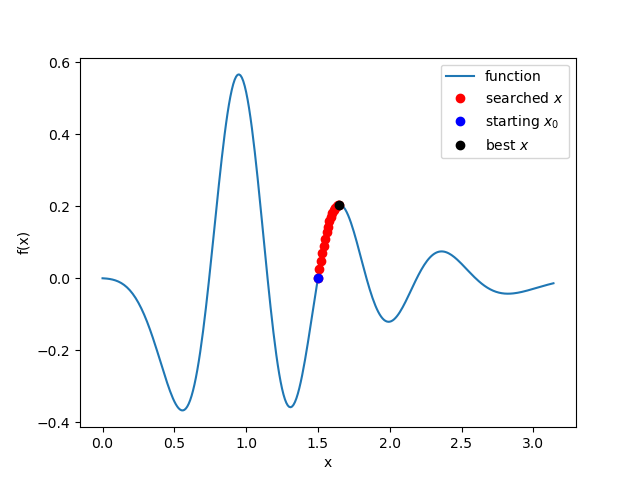
\includegraphics[width=80mm]{c:/program_code/LaTeX/OPT/class2/hillclimib_p3d_0_3.141592653589793_0.01_1.5.png}
    \caption{(2)式を探索間隔$0.01$,探索範囲$[0,\pi]$,初期値$1.5$で山登り探索を行った結果}
    \label{hp0p0.011.5}
\end{figure}

この図\ref{hp0p0.011.5}の結果では$f(1.6500000000000001)=0.20434990607375797$となり、その前の図\ref{hp0p0.010.6}や図\ref{hp0p0.011.2}
の結果とは異なる最大値が出た。この結果は全探索では出ないものであり、これが山登り探索での課題となることがわかる。

山登り探索では探索の初期値を適切に設定しなければ、このような探索範囲の最大値ではなく、極大値、すなわち局所的な最大値を取ってしまうことになることが分かる。

\subsubsection{探索範囲の変更}
ここで探索の範囲を$[-2,-1.1]$,探索の初期値を$-1.3$に変更してソースコード\ref{ex},\ref{hill}を実行した結果を以下図\ref{he-2-1.10.01-1.3},\ref{hp-2-1.10.01-1.3}にそれぞれ示す。
\begin{figure}[h]
    \centering
    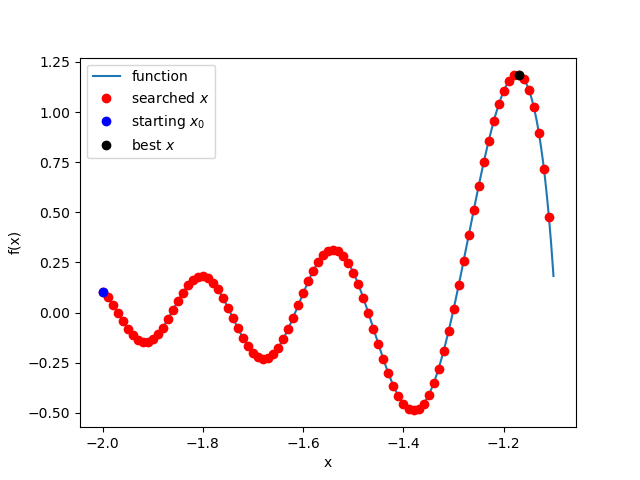
\includegraphics[width=80mm]{c:/program_code/LaTeX/OPT/class2/exsearch_p3d_-2_-1.1_0.01.png}
    \caption{(2)式を探索間隔$0.01$,探索範囲$[-2,-1.1]$で全探索を行った結果}
    \label{he-2-1.10.01-1.3}
\end{figure}
\begin{figure}[h]
    \centering
    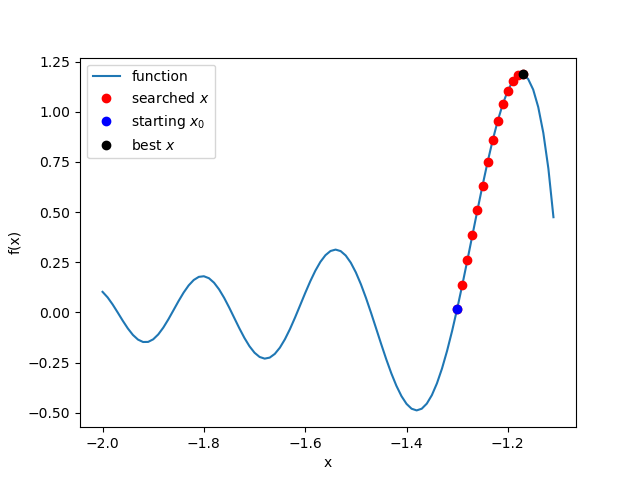
\includegraphics[width=80mm]{c:/program_code/LaTeX/OPT/class2/hillclimib_p3d_-2_-1.1_0.01_-1.3.png}
    \caption{(2)式を探索間隔$0.01$,探索範囲$[-2,-1.1]$,初期値$-1.3$で山登り探索を行った結果}
    \label{hp-2-1.10.01-1.3}
\end{figure}

この図では先ほどと探索範囲を変更しているためまた別の結果が出ている。探索範囲が$[0,\pi]$だったときの最大値が$f(0.9500000000000006)=0.5658344662199044$
であったのに対し、この範囲では$f(-1.17)=1.1863679068107829$となり、より大きな値が得られている。

このように探索範囲を変更すると関数により得られる最大値が変化することが分かる。

\subsection{2変数関数}
2変数関数での探索は、図では出力せず、textファイルでの出力とした。
ソースコード\ref{ex3d}を用い、関数は式(3)、探索範囲は$[(0,0),(\pi,\pi)]$,探索の間隔を$0.01$としたときの結果を以下ソースコード\ref{resex3d}に示す。
\begin{lstlisting}[caption={exsearch3d\_sin\_(0, 0)\_(3.14, 3.14)\_0.01.csv},label=resex3d]
    1: f([0, 0.01]): 0.009999833334166664
    2: f([0, 0.02]): 0.01999866669333308
    3: f([0, 0.03]): 0.02999550020249566
    4: f([0, 0.04]): 0.03998933418663416
    ~
    99245: f([3.139999999999977, 3.149999999999977]): -0.006814594450615605
    best: f([1.5700000000000012, 1.5700000000000012]): 1.9999993658636692
\end{lstlisting}
ソースコード\ref{resex3d}では計算回数約10万回の全探索で最大値の$f([1.5700000000000012, 1.5700000000000012])=1.9999993658636692$
が得られている。
2変数関数にすることで探索する$x$の値が2乗分多くなることでこのような結果になっている。

続いてソースコード\ref{hill3d}を用い、関数と探索範囲、間隔はそのまま、初期値を$(0.6,0.6)$としたときの結果をソースコード\ref{reshill3d}に示す。
\begin{lstlisting}[caption={hillclimib3d\_sin\_(0, 0)\_(3.14, 3.14)\_0.01\_(0.6 0.6).csv},label=reshill3d]
    1: f([0.62 0.62]): 0.5810351605373051
    2: f([0.63 0.63]): 0.5891447579422695
    3: f([0.64 0.64]): 0.5971954413623921
    4: f([0.65 0.65]): 0.6051864057360395
    ~
    95: f([1.56 1.56]): 0.9999417202299663
    96: f([1.57 1.57]): 0.9999996829318346
\end{lstlisting}
こちらの結果では計算回数95回とかなり抑えられた状態で最大値が得られている。ただソースコード\ref{hill3d}を見ると探索の方向が8方向となっており
この方向にこの範囲での最大値がない関数では、この方法が取れないことが考えられる。

\section{ソースコード}

\lstinputlisting[language=c,caption=exhaustive\_search.py, label=ex]{C:/Program_Code/Python/OPT/Class2/exhaustive_search.py}
\lstinputlisting[caption=hill\_climbing.py, label=hill]{C:/Program_Code/Python/OPT/Class2/hill_climbing.py}
\lstinputlisting[caption=exhaustive\_search\_3d.py, label=ex3d]{C:/Program_Code/Python/OPT/Class2/exhaustive_search_3d.py}
\lstinputlisting[caption=hill\_climbing\_3d.py, label=hill3d]{C:/Program_Code/Python/OPT/Class2/hill_climbing_3d.py}

\end{document}